\documentclass[11pt]{article}
\usepackage{graphicx}
\usepackage{fancyhdr}
\usepackage{wrapfig}
\usepackage{hyperref}
\usepackage{tabularx}

\addtolength{\textwidth}{0.2cm}
\setlength{\parskip}{13pt}
\setlength{\parindent}{0.0cm}
\linespread{1.5}

\pagestyle{fancy}
\fancyhf{}
\rhead{TP - Cipullo, Sullivan}
\lhead{Probalidad y Estad\'istica}
\rfoot{\vspace{1cm} \thepage}

\renewcommand*\contentsname{\LARGE Índice}

\begin{document}

\begin{titlepage}
    \begin{center}
        \vfill
        \vfill
            \vspace{0.7cm}
            \noindent\textbf{\Huge Trabajo Pr\'actico}\par
            \noindent\textbf{\Huge Estad\'istica Descriptiva}\par
            \vspace{.5cm}
        \vfill
        \noindent \textbf{\huge Alumnas:}\par
        \vspace{.5cm}
        \noindent \textbf{\Large Cipullo, In\'es}\par
        \noindent \textbf{\Large Sullivan, Katherine}\par
 
        \vfill
        \large Universidad Nacional de Rosario \par
        \noindent\large 2021
    \end{center}
\end{titlepage}
\par

El presente informe tiene como objetivo la exposici\'on de un an\'alisis estad\'istico descriptivo
sobre los datos recopilados del sistema de bicicletas compartidas de la Ciudad de Buenos Aires, EcoBici.

\section{Sobre los datos}
Los datos utilizados se encontraban divididos en dos unidades de an\'alisis diferentes: una correspondiente
a la informaci\'on sobre los usuarios del sistema en el a\~{n}o 2020, y la otra, a la informaci\'on sobre los recorridos 
realizados por los mismos, en el a\~{n}o 2020.
\par
La informaci\'on recibida para la realizaci\'on del trabajo constituye una muestra aleatoria 
de las observaciones totales registradas por el Ministerio de Desarrollo Urbano y Transporte de la
Ciudad de Buenos Aires, disponibles en {\small \url{https://data.buenosaires.gob.ar/dataset/estaciones-bicicletas-publicas}}.
\par
Todos los datos y gr\'aficos presentados a continuaci\'on provienen de esta misma y \'unica fuente.

\section{Sobre las variables}
Como fue mencionado en la secci\'on anterior, la informaci\'on se encontraba dividida en dos unidades de an\'alisis.
Cada una de ellas presenta diferentes variables que ser\'an el objeto de inter\'es de este informe.
\par
En la primer unidad (referida a informaci\'on de usuario) se cuenta con tres variables: ID de usuario 
(n\'umero de 6 d\'igitos que identifica un usuario), g\'enero de usuario (pudiendo tomar las categor\'ias femenino, masculino y otro) y
edad de usuario (representada en a\~{n}os).
\par
En la segunda unidad (referida a informaci\'on de recorridos) se cuenta con 5 variables: Duraci\'on del recorrido
(representada en segundos), Distancia (distancia entre la estaci\'on de origen y la de destino, representada en metros), 
D\'ia (d\'ia de la semana en el que se realizo el recorrido), Direcci\'on de origen (direcci\'on de la estaci\'on de EcoBici desde donde se inici\'o el recorrido), 
Direcci\'on de destino (direcci\'on de la estaci\'on de EcoBici desde donde finaliz\'o el recorrido). 

\section{An\'alisis univariado}

\subsection{G\'enero de usuario}

Cabe mencionar antes de proceder al an\'alisis de la variable que la categor\'ia "Otro" es el valor por defecto
al ingresar los datos de usuario, por lo tanto resulta posible que usuarios que se identifiquen con cualquiera
de las otras dos categor\'ias hayan quedado bajo la categor\'ia "Otro" por simplemente no modificar el valor por defecto.

Para comenzar el an\'alisis, se puede observar la siguiente tabla de frecuencias sobre la variable
g\'enero de usuario. 

\begin{center}
\begin{tabularx} {0.8\textwidth}{ 
    | >{\raggedright\arraybackslash}X 
    | >{\raggedleft\arraybackslash}X 
    | >{\raggedleft\arraybackslash}X | }
   \hline
   \textbf{G\'enero de usuario} & \textbf{Frecuencia absoluta} & \textbf{Frecuencia relativa} \\
   \hline
   Femenino & 38 & 0.38 \\
   \hline
   Masculino & 27 & 0.27 \\
   \hline
   Otro & 35 & 0.35 \\
   \hline \hline
   \textbf{Total} & 100 & 1.00 \\
   \hline
  \end{tabularx}
\end{center}

  Esta informaci\'on, dada la condici\'on cualitativa de la variable, se puede exponer
  en forma de gr\'afico de sectores. As\'i se puede visualizar claramente la porci\'on del
  total que representa cada valor de la variable.

  \hspace{-2.3cm}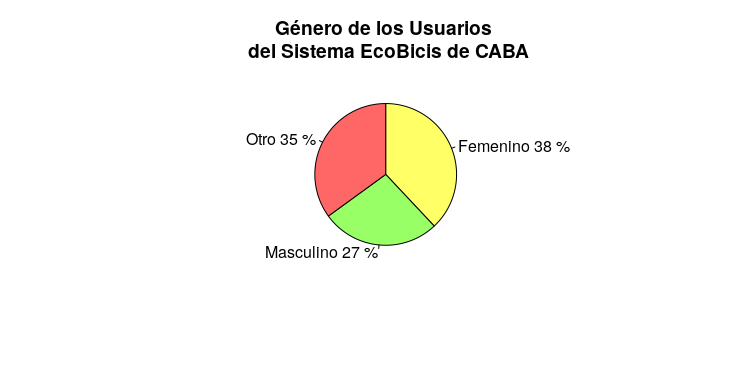
\includegraphics[scale=0.9]{PieChartGenero.png}
  \vspace{-3cm}

  De lo descripto se puede observar que las categor\'ias se encuentran bastante uniformemente
  divididas.

  \subsection{Edad de usuario}

  Para el an\'alisis de frecuencias de esta variable se procedi\'o a la divisi\'on de la misma en intervalos,
  quedando su tabla de frecuencais de la siguiente manera: 

    \begin{tabularx} {0.8\textwidth}{ 
        | >{\raggedright\arraybackslash}X 
        | >{\raggedleft\arraybackslash}X 
        | >{\raggedleft\arraybackslash}X 
        | >{\raggedleft\arraybackslash}X 
        | >{\raggedleft\arraybackslash}X |}
       \hline
       \textbf{Edad de usuario} & \textbf{Frecuencia absoluta} & \textbf{Frecuencia relativa} & \textbf{Frecuencia absoluta acumulada} & \textbf{Frecuencia relativa acumulada} \\
       \hline
       [18,23) & 16 & 0.16 & 16 & 0.16 \\
       \hline
       [23,28) & 15 & 0.15 & 31 & 0.31 \\
       \hline
       [28,33) & 27 & 0.27 & 58 & 0.59 \\
       \hline \hline
       \textbf{Total} & 100 & 1.00 \\
       \hline
      \end{tabularx}
    hacer tablita en otro tex con letra mas chqiuita y dibujarla aca




\end{document}